\chapter{Einf�hrung}
\label{chapter:Introduction}

Seit langem herrscht in Politik und Gesellschaft Uneinigkeit �ber die Auswirkungen von Gewaltdarstellungen in
Computerspielen. Trotzdem sind solche stets in einigen Spielen enthalten gewesen. Besonders das Genre der Shooter ist f�r
seine detaillierten und intensiven Gewaltdarstellungen bekannt, der Anteil an Spielen mit hohen Altersbeschr�nkungen ist
darin besonders hoch (siehe Abb. \ref{figure:stigmafreigaben}). Dennoch definiert sich dieses Genre - entgegen der oft kritischen
�ffentlichen Meinung - nicht, oder zumindest nicht ausschlie�lich �ber die enthaltenen Gewaltdarstellungen.\\

\begin{figure}[htbp]
\centering
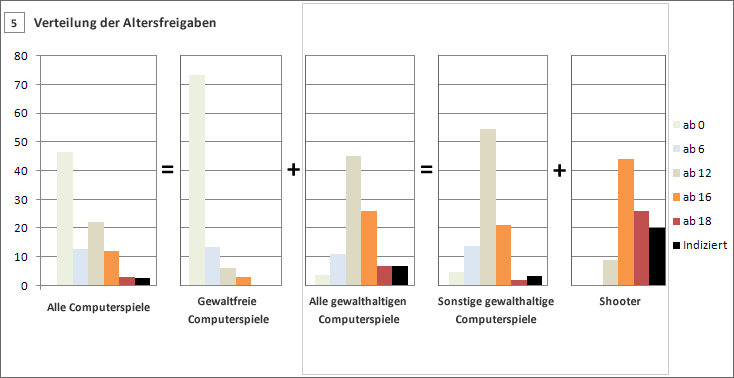
\includegraphics[width=0.8\textwidth]{images/stigmafreigaben}
\caption[Statistik der USK-Altersfreigaben nach Genres seit 1994]{Statistik der USK-Altersfreigaben nach Genres seit 1994\footnotemark}
\label{figure:stigmafreigaben}
\end{figure}
\footnotetext{Quelle: http://stigma-videospiele.de/wordpress/rechtslage/statistiken/}

\section{Zielsetzung}
Ziel dieser Arbeit ist die Analyse des Genres Multiplayer-Taktik-Shooter und die Erarbeitung eines Konzepts f�r einen
gewaltfreien Genrevertreter. Es soll gezeigt werden, dass das Spielprinzip des Shooters auch ohne Gewaltdarstellungen,
speziell ohne Schie�en auf und T�ten von Gegnern, funktioniert. Dazu sollen zum Einen die Eigenschaften, in denen sich
der Shooter au�er dem Schie�en noch von anderen Genres unterscheidet und damit selbst definiert, identifiziert und
verwendet werden. Zum Anderen sollen M�glichkeiten f�r neue Spielelemente gefunden und untersucht werden, die eine
eventuell entstehende L�cke im Konzept durch den Wegfall des Elements "`Schie�en"' f�llen oder ausgleichen k�nnen.\\

Es soll also eine M�glichkeit aufgezeigt werden, ein gutes Spiel zu entwickeln, das alle Eigenschaften und Elemente des
Shooters hat, die mit dem gewaltfreien Grundsatz vereinbar sind und somit das gleiche Klientel zufriedenstellt.

\begin{center}
Shooter - Schie�en + X $\rightarrow$ Spielqualit�t
\end{center}

Dabei ist mit Spielqualit�t Spielspa�, Motivation und Schwierigkeit gemeint, die an den Erwartungen von Shooterspielern
gemessen werden. Der Platzhalter X steht f�r Spielemente, die neu hinzugef�gt werden. Solche sollen in dieser Arbeit
gefunden und erprobt werden.
